\documentclass[11pt, landscape]{article}
\usepackage[a4paper, margin=0.8in]{geometry}
\usepackage{amsmath}
\usepackage{xcolor}
\usepackage{circuitikz}
\usepackage{enumitem}
\usepackage{graphicx}

% 设置无衬线字体以模仿幻灯片风格
\renewcommand{\familydefault}{\sfdefault}

\begin{document}

% 标题
\noindent{\Huge \textbf{Difference Amplifier Reference Voltage}}\\[0.8cm]

\begin{minipage}[t]{0.48\textwidth}
    % 左侧文本部分
    \begin{itemize}[itemsep=1.5ex, leftmargin=*]
        \item \Large For \textcolor{red}{single-ended power supply applications}, the \textcolor{red}{DC output} common-mode level is \textcolor{red}{set by $V_{REF}$}
        \item If $V_{REF}$ is equal to the DC input common-mode, in the absence of an AC signal the current through $R_1$ and $R_2$ is zero and the output voltage is also $V_{REF}$
        \item If the current required by $V_{REF}$ is small, it can be set by a voltage divider
        \item However, many applications may require a more stable voltage, necessitating a low-impedance voltage for $V_{REF}$ (e.g. an additional opamp)
    \end{itemize}
    
    \vspace{4cm}
    \textcolor{gray}{\small EE (P) 538 Lecture 5 addendum \hspace{3cm} Mahmood Hameed}
\end{minipage}%
\hfill
\begin{minipage}[t]{0.48\textwidth}
    \centering
    
    % 右侧上部：标准差分放大器电路
    \begin{circuitikz}[scale=0.9, transform shape, thick]
        \draw
        (0,0) node[op amp] (opamp) {}
        % 反相输入端
        (opamp.-) to[R, l_=$R_1$, o-] (-3, 0.5) coordinate(Vmin) node[left] {$-$}
        % 同相输入端
        (opamp.+) to[R, l_=$R_1$, o-] (-3, -0.5) coordinate(Vplus) node[left] {$+$}
        
        % Vid 标记
        (Vmin) node[above=0.3cm, xshift=-0.5cm] {$V_{id}$}
        (-3.2, 0.5) -- (-3.5, 0.5) -- (-3.5, -0.5) -- (-3.2, -0.5)
        
        % 反馈回路 R2
        (opamp.-) -- ++(0,1.5) coordinate(tmp) to[R, l=$R_2$] (tmp -| opamp.out) -| (opamp.out)
        
        % 输出端
        (opamp.out) to[short, -o] ++(0.5,0) node[right] {$V_o$}
        
        % 同相端 R2 到 V_REF
        (opamp.+) to[R, l=$R_2$] ++(0,-1.5) node[ocirc] {} node[below] {$V_{REF}$}
        ;
    \end{circuitikz}

    \vspace{0.8cm}
    
    % 右侧中部：核心公式框
    \framebox{
        \rule{0pt}{1.2cm} % 增加框内上下边距
        \hspace{0.5cm}
        \huge $\displaystyle V_o = V_{REF} + \frac{R_2}{R_1} V_{id}$
        \hspace{0.5cm}
    }

    \vspace{0.8cm}
    
    % 右侧下部：手写部分的数字化重绘
    \setlength{\fboxsep}{10pt}
    \framebox{
        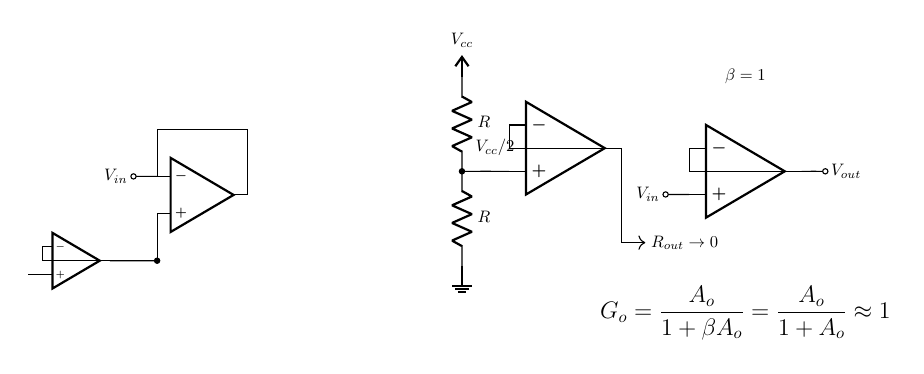
\begin{tikzpicture}[scale=0.6, transform shape]
            % --- 子电路 1：差分放大器接跟随器草图 ---
            \draw (-1.5, 0.5) node[op amp, scale=0.8] (op1) {};
            \draw (op1.-) to[short,-o] ++(-0.5,0) node[left]{$V_{in}$};
            \draw (op1.-) -- ++(0,1) -| (op1.out);
            \draw (op1.+) -- ++(0,-1) coordinate(vref_node);
            \draw (vref_node) to[short, *-] ++(-1,0) node[op amp, anchor=out, scale=0.6] (buf_left) {};
            \draw (buf_left.-) |- (buf_left.out);
            \draw (buf_left.+) -- ++(-0.3,0);
            
            % --- 子电路 2：Vcc 分压及低阻抗缓冲器 ---
            \draw (4, 3) node[vcc]{$V_{cc}$} to[R, l=$R$] (4,1) coordinate(mid) to[R, l=$R$] (4,-1) node[ground]{};
            \draw (mid) to[short, *-] ++(1,0) node[op amp, anchor=+] (buf_mid) {};
            \draw (buf_mid.-) |- (buf_mid.out);
            \node at (4.7, 1.5) {$V_{cc}/2$};
            \draw[->] (buf_mid.out) -- ++(0,-1.5) |- ++(0.5,-0.5) node[right]{$R_{out} \rightarrow 0$};

            % --- 子电路 3：跟随器增益推导 ---
            \draw (10,1) node[op amp] (buf_right) {};
            \draw (buf_right.-) |- (buf_right.out);
            \draw (buf_right.+) to[short, -o] ++(-0.5,0) node[left]{$V_{in}$};
            \draw (buf_right.out) to[short, -o] ++(0.5,0) node[right]{$V_{out}$};
            \node at (10, 3) {$\beta = 1$};
            \node at (10, -2) {\Large $\displaystyle G_o = \frac{A_o}{1+\beta A_o} = \frac{A_o}{1+A_o} \approx 1$};
        \end{tikzpicture}
    }
\end{minipage}

\end{document}